\section[Erkenntnisse]{Erkenntnisse}
\label{sec:erkenntnisse}

\subsection{Daten}
\label{sec:erkenntnisseDaten}
Für unsere Anwendung ist der GTFS Datentyp dem HRDF Datentyp aus mehreren Gründen überlegen.
\begin{enumerate}
	\item Alle zuvor genannten Programme basieren auf dem GTFS-Datentyp. Dies führt
\end{enumerate}



\subsection{Algorithmen}
\label{sec:erkenntnisseAlgorithmen}
Alle von uns genannten Algorithmen wurden schon für Journey Planner verwendet. In den Papers des RAPTORS und des CSA wurden jeweils experimentelle Vergleiche mit Dijkstra basierten Algorithmen gezogen. In allen Testfällen hatten die Dijkstra basierten Algorithmen mindestens doppelt so lange Query-Zeiten. ~\cite{csa} ~\cite{raptor}

Der RAPTOR-Algorithmus und der CSA sind sich in Vorgehen und Effizienz sehr ähnlich. Es gibt jedoch mehr Daten aus Experimenten für den CSA. Hannah Bast hat schon einen auf CSA und Transfer Pattern basierten Test mit dem Schweizer Schienennetz durchgeführt. Ihre Implementation hatte Query-Zeiten von wenigen Millisekunden. Dadurch können wir uns sicher sein, dass der CSA mit den Schweizer Daten kompatibel ist und genügend Skalierbarkeit mitbringt.~\cite{transferpatterns_esa}

Der CSA ist für unsere Arbeit am besten geeignet. Sollte jedoch durch andere Faktoren der RAPTOR-Algorithmus verlangt werden ist dieser auch akzeptabel.


\subsection{Programme}
\label{sec:erkenntnisseProgramme}
Die drei Programme Traintickets.to, OTP und R5 wurden in Betracht gezogen. 

R5 basiert zwar auf dem modernen RAPTOR Algorithmus, ist jedoch nicht für unser Projekt geeignet. Der Programmcode steht unter einer MIT-Lizenz. R5 wird von der Firma Conveyal ~\cite{conveyal} entwickelt. Wenn wir mit unserem Projekt auf das R5 Programm aufbauen, so besteht keine Chance dass unser Code in das Originalprogramm integriert wird.

Die beiden Programme Traintickets.to und OpenTripPlanner wurden genauer betrachtet. Die Programmierer beider Programme wurden von uns angeschrieben. Wir posteten eine Anfrage in die OTP Developer Mailing. Darin fragten wir ob sie zurzeit an einer Implementation des CSA in ihrem Programm arbeiten und wie sie zu der Idee unseres Projektes stehen. Nach nur kurzer Zeit bekamen wir eine Antwort. Eine Integration des CSA ist zurzeit nicht geplant. Projekte von neuen Personen sind gerne gesehen, jedoch wird der Code nur in das Hauptprogramm übernommen, wenn  das OpenSource-Gremium den Code als gut erachtet. Dazu muss der Code den Programmrichtlinien entsprechen und der Strategie des OTP entsprechen. Die Strategie des OTP liegt darin, dass sie nicht ausschliesslich auf die schnellste Lösung setzen. Wichtiger ist, dass das Programm in Echtzeit auf Verspätungen und Fahrplanänderungen reagieren kann. Wir haben auch Linus Norton von Traintickets.to angeschrieben, konnten jedoch keine Antwort erhalten. 

Um die Kompatibilität der Programme mit dem Schweizer System überprüfen versuchten wir die Programme mit den Schweitzer GTFS-Daten zu betreiben. Traintickets.to lies sich nicht ohne weiteres auf das Schweizer System anwenden. Die GTFS-Daten konnten zwar in die für den CSA benötigte Form umgewandelt werden, jedoch funktionierte der darauffolgende CSA nicht. Wir konnten das Problem im Rahmen des Fachmodules leider nicht lokalisieren. Jedoch ist es von der Skalierbarkeit her möglich das Programm auf einer landesweiten Basis zu implementieren, das es zurzeit auf dem Zugnetzwerk des United Kingodms aufbaut. Auch die Implementation des OTP führte zu Problemen. Die Ausführung funktioniert mit GTFS-Daten, welche älter als der 27.09.2017 sind. Mit neueren GTFS-Files schlägt sie jedoch fehl. Wir konnten das Problem finden. Die SBB hat einige der Routen mit dem Routetype 1700 Miscellaneous bezeichnet. Das OTP Programm beachtete diesen Route-Type nicht, obwohl er GTFS konform ist. Wir meldeten das Problem an die Development-Mailing-List wo man uns mitteilte, dass dieser Typ nicht unterstützt wird, da er nicht eindeutig einem Route-Type zugeordnet werden kann. Wenn wir OTP verwenden müssen wir dies für das Schweizer System selber implementieren. Die älteren GTFS-Daten funktionieren, da die SBB vor dem 27.09.2017 mit den Alten Route-Types arbeiteten und so den Route-Type 1700 nicht verwendeten. Die inplementation an sich funktionierte ohne Probleme und es konnten sogar die Schweitzer OpenStreetMap-Daten integriert werden.

\begin{figure}[]
	\centering
	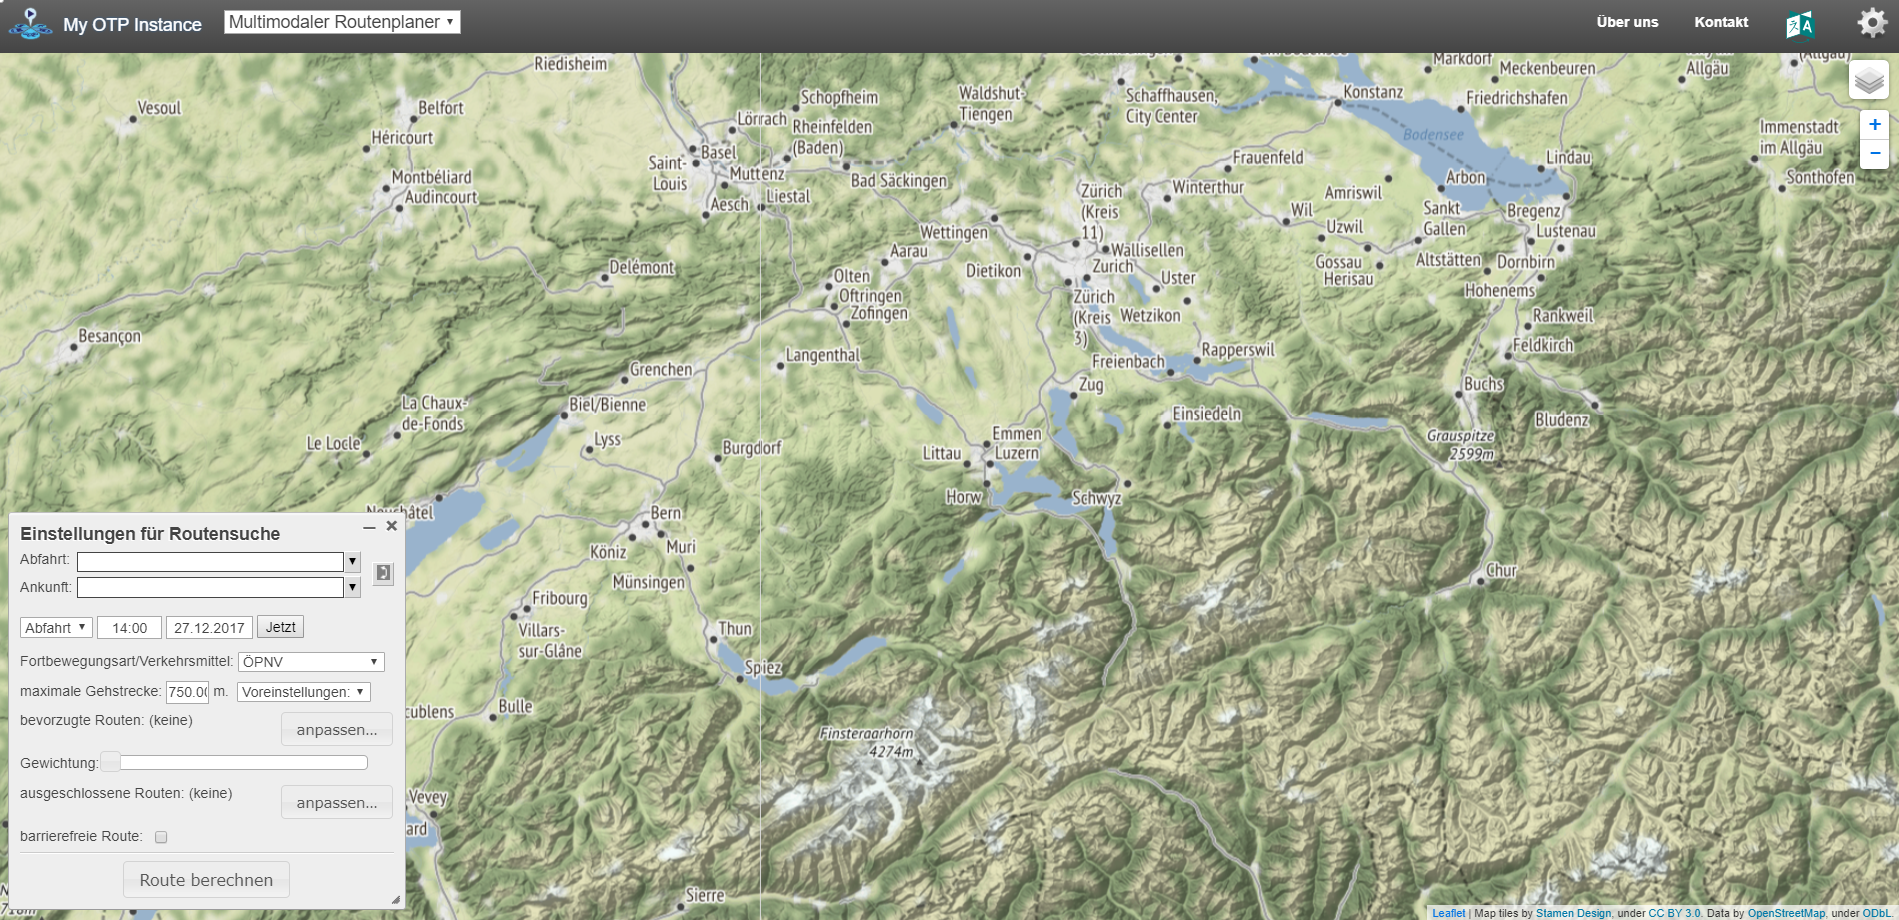
\includegraphics[width=16cm]{OTP.png}
	\caption{Implementation des OTP mit den Schweitzer Daten}
	\label{fig:OTP}
\end{figure}

Wir verglichen die Programmstrukturen der beiden Programme. Traintickets.to besitzt einige Strukturprobleme. Linus Norton selbst sagte: 'The connection scan algorithm is inherently imperative and does not port well to Scala' (Linus Norton ~\cite{traintickets_git_pattern}) Es ist in mehrere Programme aufgeteilt welche jeweils Teilaufgaben übernehmen. OTP besitzt einen sehr gut strukturierten Programmcode. Es ist nach Funktionen in verschiedene Ordner aufgeteilt, welche die jeweiligen Funktionen für die Aufgabe enthalten. Das Problem hierbei ist, dass OTP von mehr als 100 verschiedenen Entwicklern programmiert wurde. Es wurden schon mehr als 10'000 Commits durchgeführt. ~\cite{otp_website} Dadurch wird für uns das verstehen des Programmes trotz der guten Struktur viel Zeit in Anspruch nehmen. 

Aus diesen Erkenntnissen zogen wir, dass das OTP-Programm besser als Grundlage für unsere Bachelorarbeit geeignet ist. Es basiert nicht auf dem CSA. Wir werden den CSA für das OTP implementieren und dem OpenSource Gremium unsere Ergebnisse präsentieren, welche sie dann implementieren oder als Forschungswerte werte verwenden können.
 

